\documentclass[serif,xcolor=pdftex,dvipsnames,table,hyperref={bookmarks=false,breaklinks}]{beamer}

%%%%%%%%%%%%%%%%
% Change the macros below to configure the title slides
% for your course.
\newcommand{\coursename}{COMPSCI 589}
\newcommand{\instructor}{Benjamin M. Marlin}
\newcommand{\university}{University of Massachusetts Amherst}
\newcommand{\department}{College of Information and Computer Sciences}
%%%%%%%%%%%%%%%%


\newcommand{\settitlecard}[2]{
  \title[\coursename  Lecture #1] 
    {\coursename \\ Lecture #1: #2}
     \author[\instructor]{\instructor}
     \institute[\university]{
     \department\\
     \university
   }
\date{}
}

\newcommand{\maketitlepage}{
  \begin{frame}
  \titlepage
  \center{
    %If you use the slides unmodified, retain the attribution below
    \tiny{Slides by Benjamin M. Marlin (marlin@cs.umass.edu). \\
    \vspace{-1em}Created with support from National Science Foundation Award\# IIS-1350522. 
    %If you modify the slides, please retain the alternate attribution below
    %\tiny{Based on slides by Benjamin M. Marlin (marlin@cs.umass.edu). \\    
    %\vspace{-1em}Created with support from National Science Foundation Award\# IIS-1350522. 
    }                                              
  }  
  \end{frame}
}

\AtBeginSection[]
{
  \begin{frame}<beamer>{Outline}
    \tableofcontents[currentsection,subsectionstyle=hide]
  \end{frame}
}


\newcommand{\cut}[1]{}

\newcommand{\iconbox}[4]{
  \only<#1-#2>{
    \begin{columns}[T]
      \column{0.5in}
           \includegraphics[width=0.5in]{#3}
       \column{3.7in}
            #4
    \end{columns}
    \medskip
    \medskip
    \medskip
  }
}

\mode<presentation>{
  \usepackage{../beamertheme589theme}
  \setbeamercovered{invisible}
}

\mode<handout>{
  \usepackage{../beamertheme589theme}
  \setbeamercovered{transparent}
}


\usepackage[english]{babel}
\usepackage[latin1]{inputenc}
\usepackage{times}
\usepackage[T1]{fontenc}
\usepackage{amsmath}
\usepackage{amssymb}
\usepackage[noend]{algorithmic}
\usepackage{algorithm}
\usepackage{listings}

\renewcommand\mathfamilydefault{\rmdefault}

\newcommand{\setA}{\mathcal{A}}
\newcommand{\setB}{\mathcal{B}}
\newcommand{\setS}{\mathcal{S}}
\newcommand{\setV}{\mathcal{V}}
\DeclareMathOperator*{\union}{\bigcup}
\DeclareMathOperator*{\intersection}{\bigcap}
\DeclareMathOperator*{\Val}{Val}
\newcommand{\mbf}[1]{{\mathbf{#1}}}
\DeclareMathOperator*{\argmax}{arg\,max}
\DeclareMathOperator*{\argmin}{arg\,min}
\DeclareMathOperator*{\sign}{sign}
\newcommand{\deriv}[2]{\frac{\partial{#1}}{\partial{#2}}}


\settitlecard{11}{KOLS and Gaussian Process Regression}

\begin{document}

\maketitlepage

\section{SVR and KOLS}
\subsection{foo}

\begin{frame}[t]{Support Vector Regression}

\begin{itemize}
\item Support Vector Regression (SVR) is the generalization of SVMs to the case of regression.

\pause \item As with SVMs, SVR is a linear model trained using a different 
objective function. In this case, the \textit{epsilon insensitive loss}.
\end{itemize}
\pause
\center
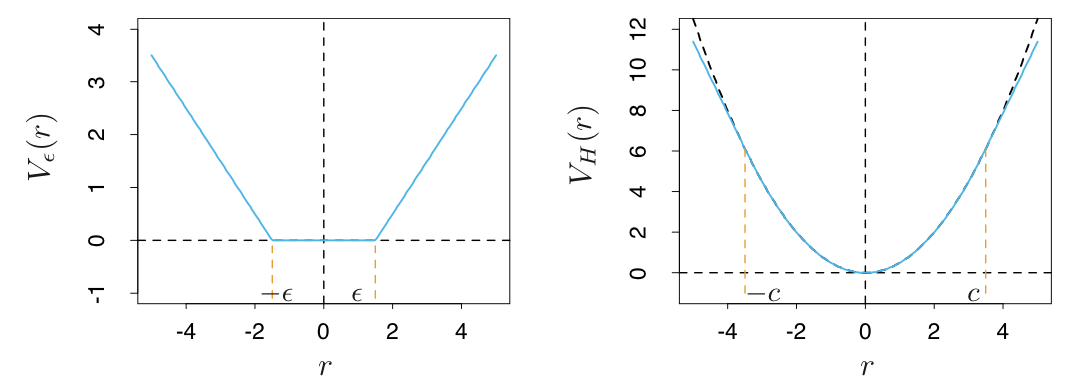
\includegraphics[width=4in]{../Figures/svr_loss.png}

\end{frame}


\begin{frame}[t]{Kernelization}

Using the same representer theorem used in classification, it can be shown that

$$f_{Lin}(\mbf{x}) = \mbf{x}\mbf{w}^*+b* = \sum_{i=1}^N \alpha_i<\mbf{x},\mbf{x}_i> + \sum_{i=1}^N \alpha_i<1,\mbf{x}_i>$$

\pause This can again be generalized using kernels to allow for non-linear models:
$$f_{Lin}(\mbf{x}) = \mbf{x}\mbf{w}^*+b* = \sum_{i=1}^N \alpha_iK(\mbf{x},\mbf{x}_i)$$

\pause Let's have a look at how this model works in more detail.

\end{frame}

\begin{frame}[t]{What About Probabilities?}

\begin{itemize}
\item An additional drawback of SVR is that it isn't probabilistic.

\pause\item For many applications like weather prediction and stock 
market forecasting, we might like the model to predict both a 
mean value and a confidence interval or standard deviation.

\pause\item \textbf{Question:} How can we define a flexible regression model 
like SVR, but with probabilistic outputs?
\end{itemize}

\end{frame}

\begin{frame}[t]{OLS Regression as a Probabilistic Model}

Recall that the ordinary least squares solution to linear regression
is equivalent to optimizing the following probabilistic model
where $\sigma^2$ is the noise variance.

\pause
\begin{align*}
P(y|\mbf{x}) = \mathcal{N}(y;\mbf{x}\mbf{w}, \sigma^2)
             = 
\frac{1}{\sqrt{2\pi\sigma^2}}\exp\left(-\frac{1}{2\sigma^2}(y-\mbf{x}\mbf{w}
)^2\right)
\end{align*}

\end{frame}

\begin{frame}[t]{Parameter Estimates}

The solution for the parameter estimates is:

\begin{align}
\mbf{w}_* & = (\mbf{X}^T\mbf{X})^{-1}\mbf{X}^T\mbf{Y}\\
\sigma^2_*  & = \frac{1}{N}\sum_{n=1}^N (y_n - \mbf{x}_n\mbf{w})^2
\end{align}

\pause Note that learning this model estimates both the regression
weights $\mbf{w}$ and the residual noise variance $\sigma^2$.

\end{frame}

\begin{frame}[t]{Kernelized OLS Regression}

Just as with SVR, the OLS solution can be written in terms of inner products 
between data cases and the representer theorem can be used to obtain a 
kernelized form of the model where:

\pause
$$f_{Lin}(\mbf{x}) = \mbf{x}\mbf{w}_* = \sum_{i=1}^N 
\alpha_iK(\mbf{x},\mbf{x}_i)$$

\pause
$$\sigma^2  = \frac{1}{N}\sum_{n=1}^N (y_n - f_{Lin}(\mbf{x}_n))^2$$

\pause Let's have a look at how this model compares to SVR.

\end{frame}

\begin{frame}[t]{KOLS and Uncertainty}

\textbf{Question:} What is the problem with the uncertainty estimate coming 
from KOLS?\\[12pt]

\pause It's the same everywhere! We should have more uncertainty far from where
we have data and less uncertainty close to where we have data.

\end{frame}



\section{GPR}
\subsection{Foo}

\begin{frame}[t]{Gaussian Process Regression}

\begin{itemize}
\item Gaussian Process Regression is a kernelized probabilistic regression model
that infers a probability distribution over latent functions (a 
\textit{stochastic process}).  

\pause \item A Gaussian process regression model uses a Gaussian process prior 
over the space of functions, and a regular normal likelihood.

$$p(f) = \mathcal{GP}(f;m,\mathcal{C})\;\;\;\;\; p(y|\mbf{x},f) = 
\mathcal{N}(y;f(x),\sigma^2)$$

\pause \item A Gaussian process is characterized by a mean function 
$m(\mbf{x})$ and a covariance function (kernel function) 
$\mathcal{C}(\mbf{x},\mbf{x}')$ such that the joint distribution of the process
over any finite collection of input $\mbf{x}_1,...,\mbf{x}_n$ is multivariate 
Gaussian. 

\end{itemize}

\end{frame}

\begin{frame}[t]{Gaussian Process Regression}

The covariance function $\mathcal{C}$ defines how ``smooth'' typical
functions $f$ from the process look. Different covariance functions
and different hyper-parameters lead to favoring different types of functions.

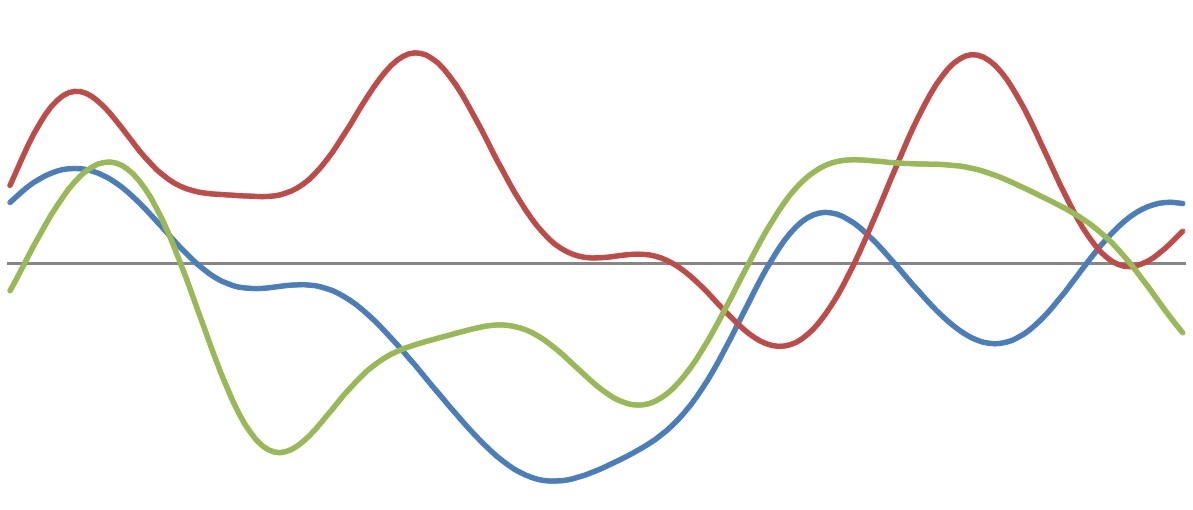
\includegraphics[width=4in]{../Figures/GPsamples1.png}

\end{frame}

\begin{frame}[t]{Gaussian Process Regression}

The covariance function $\mathcal{C}$ defines how ``smooth'' typical
functions $f$ from the process look. Different covariance functions
and different hyper-parameters lead to favoring different types of functions.

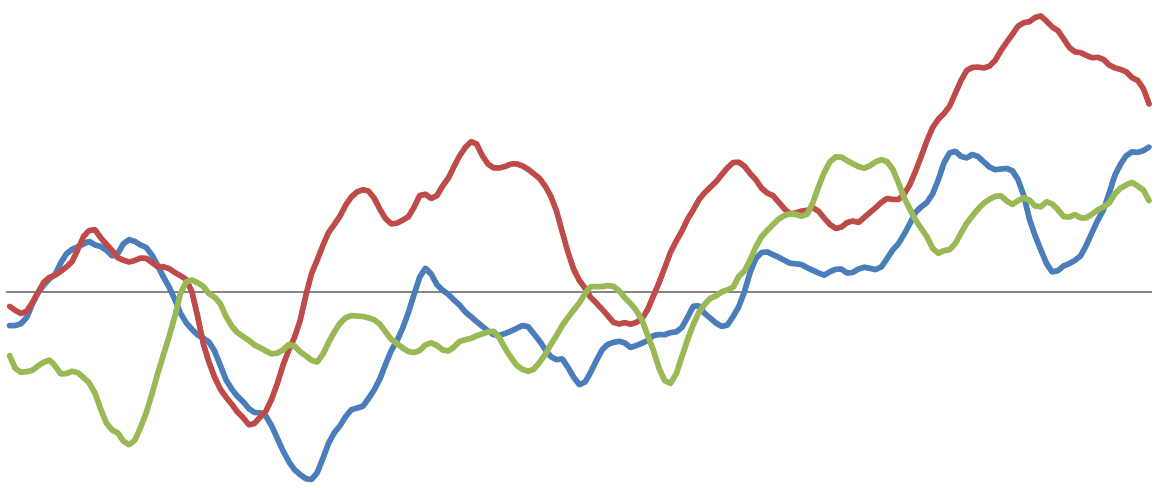
\includegraphics[width=4in]{../Figures/GPsamples2.png}

\end{frame}

\begin{frame}[t]{Gaussian Process Regression}

\begin{itemize}
\item Intuitively, the model defines the distribution $p(y|\mbf{x})$ by 
integrating over the space of all possible functions:

\pause
$$p(y|\mbf{x}) = \int 
\mathcal{N}(y;f(x),\sigma^2)\mathcal{GP}(f;m,\mathcal{C})df$$

\pause\item If we have a data set 
$\mathcal{D}=\{(y_i,\mbf{x}_i\}_{i=1:N}$, we can (conceptually) invert this 
model using Bayes rule to infer $p(f|\mathcal{D})$:

$$p(f|\mathcal{D}) = \mathcal{GP}(f;\mu_N,\mathcal{C}_N)\frac{\prod_{i=1}^N 
\mathcal{N}(y_i;f(\mbf{x}_i),\sigma^2)\mathcal{GP}(f;m,\mathcal{C})}
{\int \prod_{i=1}^N
\mathcal{N}(y_i;f(\mbf{x}_i),\sigma^2)\mathcal{GP}(f;m,\mathcal{C})df}
$$

\pause\item We can then make predictions for new points using the equation:

$$p(y|\mbf{x},\mathcal{D}) = \int 
\mathcal{N}(y;f(x),\sigma^2)\mathcal{GP}(f;\mathcal{D})df$$

\end{itemize}

\end{frame}

\begin{frame}[t]{Gaussian Process Regression}

\begin{itemize}
\item It may look like the prediction computation $p(y|\mbf{x},\mathcal{D})$ is 
impossible to actually carry out here, but it turns out to be computable in 
closed form:

\pause \item Let $\mbf{y} = [y_1,...,y_N]^T$ 

\pause \item Let $\mbf{m} = [m(\mbf{x}_1),...,m(\mbf{x}_N)]^T$ and $m_* = 
m(\mbf{x})$
\pause \item Let $\Sigma_{ij} = \mathcal{C}(\mbf{x}_i,\mbf{x}_j)$, 
$(\Sigma_*)_{i,1} = \mathcal{C}(\mbf{x}_i,\mbf{x})$ and $(\Sigma_{**}) = 
\mathcal{C}(\mbf{x},\mbf{x})$.

\pause\item We can compute the predictive distribution as follows:
\begin{align*}
  p(y|\mbf{x},\mathcal{D}) &= \mathcal{N}(y; \mu_*,\sigma^2_*)\\
  \mu_* &= m_* + \Sigma_*^T (\Sigma + \sigma^2I)^{-1} (\mbf{y} - 
\mbf{m})\\
  \sigma^2_*& = \Sigma_{**} - \Sigma_*^T (\Sigma + \sigma^2I)^{-1}\Sigma_*
\end{align*}

\pause\item Let's see what this model can do.


\end{itemize}

\end{frame}

\begin{frame}[t]{Learning}

\begin{itemize}
\item Since as a non-parametric Bayesian model, GPR has no explicit model 
parameters to learn like SVR. 

\pause\item The covariance function that defines a GP has the same 
hyper-parameters as the corresponding kernel when used in SVR.

\pause\item The hyper-parameters can be set via cross validation. They can also
be learned on training data using maximum marginal likelihood optimization.

\end{itemize}

\end{frame}

\begin{frame}[t]{Trade-Offs}

\begin{itemize}
\item The computational complexity of GPR scales with cube of the number of
input points due to inversion of the covariance matrix. This can be sped up 
using a number of approximations.

\item Unlike SVR and KOLS, GPR provides a more sensible estimate of uncertainty
that reflects the amount of data locally.

\item The likelihood function is still Gaussian; however, so the model is 
sensitive to outliers like OLS, and unlike SVR.

\item Unlike SVR, the model does not have a support vector property. This means
naive GPR implementations must retain access to all data similar to KNN. 
regression.

\end{itemize}

\end{frame}




\end{document}
